%==============================================================================
%== template for LATEX poster =================================================
%==============================================================================
%
%--A0 beamer slide-------------------------------------------------------------
\documentclass[final]{beamer}
\usepackage[orientation=portrait,size=a0,
            scale=1.25         % font scale factor
           ]{beamerposter}
           
\geometry{
  hmargin=2.5cm, % little modification of margins
}

%
\usepackage[utf8]{inputenc}
\renewcommand{\figurename}{Figura}

\linespread{1.15}
%
%==The poster style============================================================
\usetheme{sharelatex}

%==Title, date and authors of the poster=======================================
\title
[XIX Seminário de Iniciação Científica da UEFS, Outubro 2015, Feira de Santana, Bahia] % Conference
{ % Poster title
AVALIAÇÃO DE TÉCNICAS DE RECONHECIMENTO DE PADRÕES ADEQUADAS À CRIAÇÃO DE UM SISTEMA BASEADO EM GPU PARA A CLASSIFICAÇÃO DE IMAGENS MÉDICAS USADAS EM CITOPATOLOGIA RENAL
}

\author{ % Authors
Diego de Jesus Leite\inst{1}, Angelo Amâncio Duarte\inst{1}
}
\institute
[Very Large University] % General University
{
\inst{1} Universidade Estadual de Feira de Santana\\[0.3ex]
diegojleite@gmail.com, angeloduarte@ecomp.uefs.br
}
\date{\today}



\begin{document}
\begin{frame}[t]
%==============================================================================
\begin{multicols}{2}
%==============================================================================
%==The poster content==========================================================
%==============================================================================

\section{Introdução}
A computação tem se mostrado uma aliada fundamental para o processo de desenvolvimento da ciência e tecnologia. O campo de processamento de imagens e visão computacional, especialmente, tem contribuído de maneira significativa em diversas áreas do conhecimento.
\newline

Na medicina, um bom exemplo de aplicação é o desenvolvimento de sistemas de captura e processamento digital de imagens, que tem possibilitado o registro massivo de aspectos normais e patológicos nos tecidos biológicos. Outras áreas se baseiam no uso de imagens para auxílio ao diagnóstico, como é o caso da citopatologia, onde patologistas analisam alterações da morfologia celular através da análise ao microscópio de lâminas de tecido ou fluído, extraídas do órgão em análise do paciente, para o reconhecimento de padrões que indiquem a presença ou não de alguma enfermidade.
\newline

A diferenciação das variantes de doenças a partir das imagens é uma tarefa computacionalmente complexa e está longe de ser resolvida. Dentre as principais dificuldades enfrentadas, estão: a seleção do melhor conjunto de características e correta extração das mesmas, a partir das imagens obtidas.
\newline

A partir destas dificuldades, este projeto propôs o estudo e a implementação de algoritmos que pudessem auxiliar nas etapas de pré-processamento, segmentação e extração de características de imagens coletadas de lâminas de tecido renal analisadas ao microscópio.

\section{Metodologia}

Durante o tempo de desenvolvimento do projeto ocorreram encontros semanais entre os integrantes do Laboratório de Computação de Alto Desempenho (LaCAD), com o intuito de estabelecer discussões técnicas para propor soluções aos problemas enfrentados pelo projeto.
\newline

Foram utilizadas 284 amostras, durante o período de estudos e execuções de testes dos algoritmos, disponibilizadas pelo Dr. Washington Luís Conrado dos Santos, pesquisador  do Laboratório de Patologia e Biointervenção (LBPI) do Centro de Pesquisas Gonçalo Moniz da FIOCRUZ (CPqGM/FIOCRUZ).Desse montante de 284 amostras, 166 eram de imagens de glomérulos normais e 118 apresentavam algum tipo de glomerulopatia.
\newline

\section{Resultados e discussão}

Nesta seção são apresentados os resultados obtidos durante a implementação dos algoritmos responsáveis por fazer o pré-processamento, a segmentação e a extração de características das imagens presentes no conjunto de amostras.

\vskip1ex
\begin{figure}
	\centering
	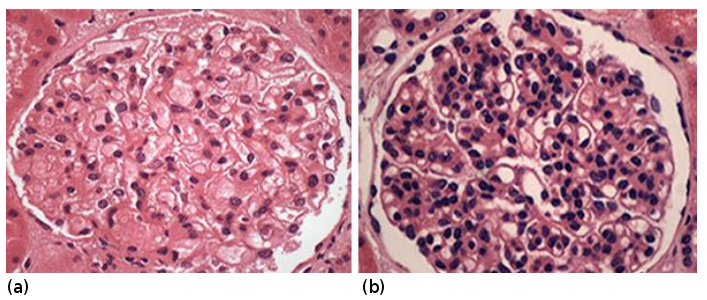
\includegraphics[width=1\columnwidth]{img1.png}
	\caption{Glomérulo normal (A) e Glomérulo com algum tipo de glomerulopatia (B).}
\end{figure}
\vskip2ex

\subsection{Pré-processamento}

\vskip1ex
\begin{figure}
	\centering
	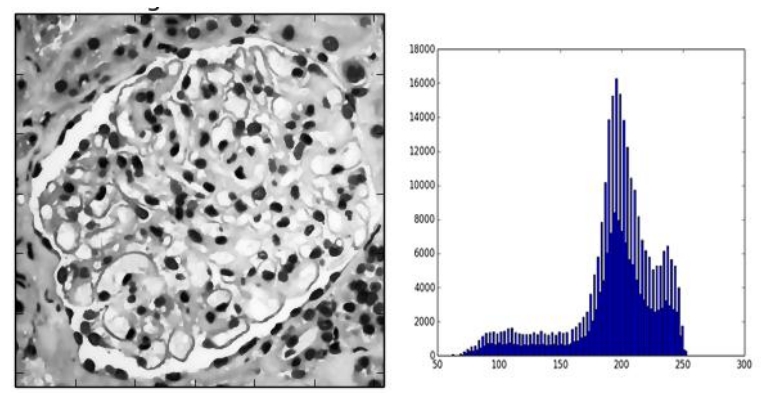
\includegraphics[width=1\columnwidth]{img2.png}
	\caption{Imagem de Glomérulo em escala de cinza e o seu histograma normalizado.}
\end{figure}
\vskip2ex

\subsection{Segmentação}

\vskip1ex
\begin{figure}
	\centering
	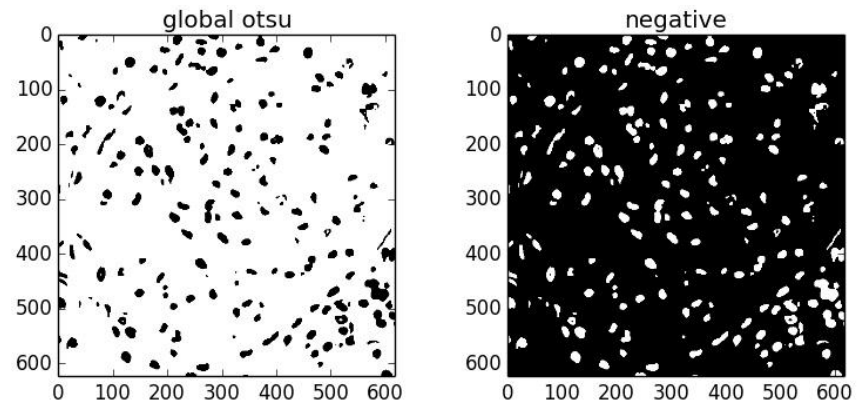
\includegraphics[width=1\columnwidth]{img3.png}
	\caption{Imagem segmentada e depois invertida.}
\end{figure}
\vskip2ex

\subsection{Extração de características}

\vskip1ex
\begin{figure}
	\centering
	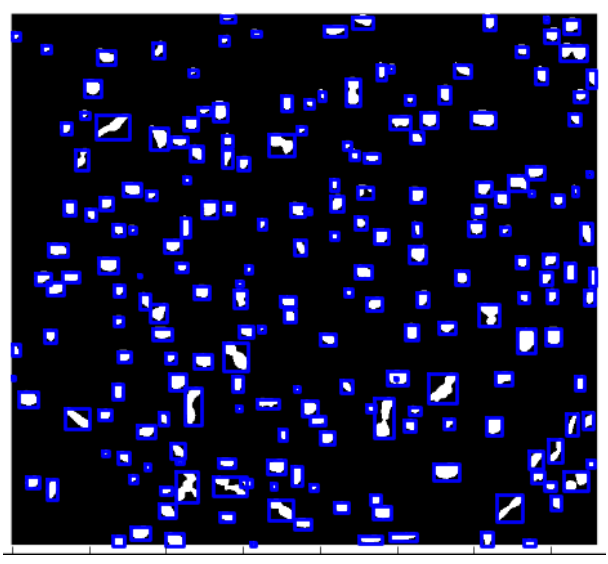
\includegraphics[width=.5\columnwidth]{img4.png}
	\caption{Núcleos localizados através do algoritmo de Blob Detection.}
\end{figure}
\vskip2ex


\section{Conclusão}

Os resultados obtidos através da pesquisa realizada, bem como as atividades desenvolvidas, foram satisfatórios, pois os algoritmos desenvolvidos durante a vigência da bolsa encontram-se em funcionamento e estão sendo utilizados no projeto PathoSpotter.
\newline

Como fruto da minha participação nas atividades do PathoSpotter, também tive a oportunidade de participar da Jornada Baiana de Patologia Hepática e Renal, em maio de 2015, sediada pelo Centro de Pesquisa Gonçalo Moniz da FIOCRUZ em Salvador, onde o PathoSpotter foi apresentado oficialmente para a comunidade científica nacional.


%==============================================================================
%==End of content==============================================================
%==============================================================================

\end{multicols}

%==============================================================================
\end{frame}
\end{document}
